\documentclass[a4paper,12pt]{article}

\usepackage[spanish]{babel}
\usepackage[utf8]{inputenc}
\usepackage{enumerate}
\usepackage{amsmath}
\usepackage{extsizes}
\usepackage{amssymb}
\usepackage{dsfont}
\usepackage{graphicx}
\usepackage{cancel}
\usepackage[usenames]{color}
\usepackage[dvipsnames]{xcolor}
\usepackage{accents}
\usepackage{flushend}
\usepackage{tikz}

\usetikzlibrary{arrows,automata}
\usepackage{multicol}
\setlength{\columnsep}{1cm}
\usepackage{listings}
\usepackage{graphics,graphicx, float} %para incluir imágenes y colocarlas



\usepackage[hidelinks]{hyperref}

\usepackage[vmargin=3cm,hmargin=3cm]{geometry}
%\setlength\parindent{0pt}

\setlength\parindent{0pt}
\setlength{\parskip}{10px}


% Carpeta con las imágenes
%\graphicspath{{}}

\begin{document}


	\begin{center}
		\LARGE{\textbf{Visión por Computador (2018-2019)} \\ Grado en Ingeniería Informática y Matemáticas \\ Universidad de Granada }
		\vspace*{2.5cm}

		\rule{\textwidth}{1.6pt}\vspace*{-\baselineskip}\vspace*{4pt}
		\rule{\textwidth}{1.6pt}\vspace*{-\baselineskip}\vspace*{2pt}
		\vspace{0.5cm}

		\Huge{Descriptores HOG en la detección de peatones}

		\vspace{0.5cm}
		\rule{\textwidth}{1.6pt}\vspace*{-\baselineskip}\vspace*{2pt}
		\rule{\textwidth}{1.6pt}\vspace*{-\baselineskip}\vspace*{4pt}

		\vspace{4cm}

\begin{figure}[h!]
	\centering
	
\includegraphics[scale=0.75]{./Imagenes/etsiit.jpeg}
	\label{fig:logoETSIIT}
\end{figure}

		\vspace{4cm}
		\large{Ignacio Aguilera Martos y Diego Asterio de Zaballa \\ \today }

	\end{center}




\newpage

\tableofcontents

\newpage

%%%%%%%%%%%%%%%%%%%%%%%%%%%%%%%%%%%%%%%%%%%%%%%%%%%%%%%%%%%%%%%%%%%%%%%%%%%%%%%%%%%%%%
%%             Descripción del problema y el enfoque que le hemos dado              %%
%%%%%%%%%%%%%%%%%%%%%%%%%%%%%%%%%%%%%%%%%%%%%%%%%%%%%%%%%%%%%%%%%%%%%%%%%%%%%%%%%%%%%%

\section{Descripción del problema y enfoque de la resolución}

En la resolución de este trabajo nos hemos planteado el siguiente problema a resolver, dada una imagen de una persona andando por la calle (un peatón), ¿cómo podemos reconocer que es un peatón?

Esta misma cuestión fue planteada por Navneet Dalal y Bill Triggs en su paper ``Histogram of Oriented Gradients for Human Detection'' en el que explican el desarrollo de unos descriptores que aplicados a su dataset de personas obtienen unos resultados muy buenos en la detección de las mismas.

Estos descriptores son los descriptores HOG o descriptores de histogramas basados en gradientes. Como veremos a lo largo del trabajo se han empleado distintas variaciones a la hora de hallar los descriptores por Dalal y Triggs, quedándonos nosotros con las elecciones que han resultado más fructíferas para ellos en su análisis.

Para comenzar hay que saber que la detección de personas es un problema difícil de abordar y que actualmente resulta muy interesante en aplicaciones por ejemplo en coches, de forma que si detecta un peatón andando por delante del vehículo este entienda que tiene que detenerse.

Las herramientas usadas en este proyecto han sido:
\begin{itemize}
	\item Python para la implementación.
	\item OpenCV y NumPy para las operaciones de los algoritmos.
	\item El módulo de SVM incluido en OpenCV para poder predecir la existencia o no de un humano en una imagen en base a los descriptores calculados.
	\item El dataset dado por los investigadores empleado en la elaboración de su artículo.
\end{itemize}

A continuación hacemos una descripción un poco más elaborada del problema propuesto.

\subsection{Problema a resolver}

El problema consiste en, dada una imagen que contiene o no un peatón, debemos determinar si es que lo contiene y además una región aproximada en la que se encuentra el mismo.

Para la elaboración de la solución del problema hemos utilizado varios ingredientes entre los que tenemos la fase de creación de descriptores y entrenamiento de la SVM y la fase de test.

En la fase de entrenamiento de los descriptores obtenemos un dataset ya formado por parte del grupo de investigación con parches de personas y con parches que no son personas todos con el mismo tamaño. De esta forma podemos obtener descriptores comparables entre sí para las imágenes positivas y negativas con lo que entrenaremos una SVM.

La segunda fase es la de test que comparte dificultad e importancia con la primera. Como explicaremos más en detalle posteriormente resolvemos el problema de dada una imagen, ¿cómo la tenemos que analizar para poder identificar si hay o no personas y dónde están? En secciones siguientes veremos que la solución adoptada ha sido una ventana deslizante con algunas modificaciones importantes cuyos parches extraídos se pasan a la SVM y se predice sobre ellos para poder detectar el área de la imagen en la que obtenemos respuestas positivas a la pregunta de si hay o no una persona.

\subsection{Descriptores HOG}

El problema mencionado anteriormente se ha enfrentado desde
distintos puntos de vista lo que ha dado lugar a diversos
descriptores. Nuestra implementación se basa en el paper de
Navneet Dalal y Bill Triggs en el que desarrollan un descriptor
basado en el gradiente de una imagen llamado descriptor HOG.
El metodo se basa en calcular los gradientes de una imagen y a
continuación construir histogramas locales basado en la
orientación de dichos gradientes.

La idea básica sobre la que se desarrolla la técnica es que las
características de forma y apariencia de un objeto de forma local
se pueden resumir gracias a la distribución de la orientación de
los gradientes de la imagen.

A continuación se describe la implementación de la técnica a
grandes rasgos. En primer lugar cada imagen se procesa con una
normalización Gamma tras un suavizado se calculan los gradientes
de la imagen. A esto le sigue que la ventana de la imagen sobre la
que se va a construir el vector de características se divide en
celdas. Estas celdas son pequeñas regiones de la imagen. En cada
una de estas celdas se calcula el histograma de la dirección de
los gradientes que en ella se encuentran. Por ultimo estas
celdas se agrupan en bloques para que sea posible normalizar los
histogramas. Finalmente, el vector de características lo conforman
los histogramas normalizados concatenados uno detrás de otro.

Conviene detallar cada uno de los pasos que se han seguido en el
proceso de construcción del descriptor.

\subsubsection{Normalización Gamma}

La fase de normalización consiste en corregir los valores de la
imagen gracias a una transformación del tipo
\[
  v_{\text{out}} = \alpha \cdot v_{\text{in}}^\beta
\]
esta transformación se aplica a cada píxel de la imagen.

\subsubsection{Computo del gradiente}

Previo al computo del gradiente se puede realizar un suavizado de
la imagen convolucionando una mascara Gaussiana. Sin embargo, los mejores resultados se alcanzan sin ese suavizado.  A continuación
se calculan las derivadas direccionales $\frac{df}{dx}$ y
$\frac{df}{dy}$ convolucionando el kernel uno dimensional
\[
  \begin{bmatrix}-1 & 0 & 1\end{bmatrix}
\]
por filas y columnas respectivamente.

\subsubsection{Generación de los histogramas}

Para generar los histogramas hace falta establecer el tamaño de las
celdas en nuestro caso son celdas $6\times 6$ píxeles. A
continuación en cada píxel de la celda se considera el gradiente de
la imagen en ese píxel. Se calcula el ángulo que forma con el eje
OX y la magnitud del gradiente. Si el ángulo $\alpha$ es mayor que
$180$ entonces se toma el ángulo $\alpha - 180$.

El gradiente de la imagen en ese píxel va a realizar un voto que
se acumulara en el histograma de la celda en la que se encuentre
dicho gradiente. El voto que realiza cada gradiente coincide con
la magnitud del propio gradiente. Para determinar sobre cuales
de las columnas del histograma se acumula el voto se utiliza el
ángulo $\theta$ del gradiente. Cada columna del histograma se
identifica con un ángulo entre 0 y 180 hay tantos ángulos como
columnas tenga el histograma (en nuestro caso 9) y están a la misma
distancia unos de otros. A continuacion se eligen los dos angulos
$\theta_i,\theta_{i+1}$ de entre los nueve mencionados anteriormente
de forma que $ \theta_i \le \theta < \theta_{i+1} $. A la columna
$i$-esima se le vota con
\[
  (1-\frac{\theta-\theta_i}{\theta_{i+1} - \theta_i})\| \nabla f (x,y)\|_2
\]
y a la $i+1$-esima con
\[
  (\frac{\theta-\theta_i}{\theta_{i+1} - \theta_i})\| \nabla f (x,y)\|_2
\]

\subsubsection{Normalización de los bloques}

A continuación las celdas se agrupan en bloques de tamaño
$3\times 3$ celdas. Los histogramas de las celdas se concatenan
juntos y el vector resultante $v$ se normaliza utilizando la
norma euclídea :
\[
  \frac{v}{\|v\|_2}
\]
En esta seccion es importante que los bloques se solapen, es
decir habra bloques que compartan celdas. Para conseguir esto
empezamos con el bloque formado por las $3\times 3$ primeras
celdas una vez esta construido y normalizado se almacena el
vector resultado y se siguen construyendo bloques. Cada bloque
en construccion se rellena con la matriz formada por las
$3\times 3$ celdas que estan un paso a la derecha. Cuando
se agota la fila cambiamos de columna. De esta forma,
recorremos toda la ventana.

En ultimo lugar los vectores que se han formado siguiendo el
procedimiento comentado arriba se concatenan. Este es el
descriptor final.

\subsection{Fases de la resolución}


\subsubsection{Procedimiento para entrenar el modelo SVM}

Las palabras del Test se han generado a partir de las imágenes de
la base de datos INRIA. Esta es la base de datos con la que se
obtuvieron por primera vez los resultados del descriptor HOG.

En primer lugar se han procesado las imágenes del test etiquetadas
como positivas. Con ese fin hemos utilizado el archivo de anotaciones
que tiene cada imagen positiva del test. Cada imagen etiquetada como
positiva tiene asociado un archivo con anotaciones en las que se almacenan
las coordenadas de cada peatón dentro de la imagen. A partir de esa
información cada peatón de la imagen se ha recortado y redimensionado
al tamaño de la ventana, es decir $64\times 128$. A este conjunto de imágenes positivas se le han añadido sus reflejadas con respecto al borde derecho de la imagen, de forma que continuamos teniendo peatones con la cabeza en la parte superior y los pies en la inferior, obteniendo el doble de ejemplos positivos a partir de los recortes.

En segundo lugar se han procesado las imágenes negativas. Para
obtener recortes de las imágenes negativas se ha recorrido el
directorio de las imágenes negativas y por cada imagen se han
obtenido $10$ recortes del tamaño considerado que se han etiquetado
como negativas. Los $10$ recortes se han elegido de forma aleatoria
dentro de las imágenes. A partir de todos esos recortes se han generado
los descriptores HOG asociados con los que se ha entrenado la SVM.

Hemos utilizado la implementación de openCV de SVM. La SVM es
lineal y tiene el mismo coeficiente C que en el paper de referencia
es decir $C = 0.01$.

Después de obtener un predictor preliminar se ha buscado dentro de las
imágenes negativas recortes de la ventana deslizante que hagan falsos
positivos. Estos se han almacenado en un directorio llamado falsos\_positivos
una vez determinados esos falsos positivos se ha reentrenado la SVM.

En total el numero de imágenes de ventanas positivas que se han
conseguido es $1237$ más sus imágenes reflejadas con respecto al borde derecho.. Para las imágenes negativas hay $10$ ventanas por
cada imagen de modo que en total son $12180$. A todo eso además se le añade
un numero considerable de falsos positivos para mejorar los resultados
de la predicción.

\subsubsection{Procedimiento para la detección de un peatón en una imagen de test}

El el paper de referencia no se discute en ningún momento el método de test utilizado por los investigadores por lo que, para que sea comparable con otras técnicas actuales, hemos empleado un método de test utilizado actualmente para medir el acierto de la detección.



El dataset INRIA tambien incluye un fichero de anotaciones en el caso en el que la imagen de Test es positiva. Como en la fase de entrenamiento las anotaciones indican el rectángulo de la imagen en el que aparece un peatón. De esta forma, una vez estimada la región en la que el predictor encuentra un peatón se puede comprobar si coincide con las regiones provistas por el fichero de anotaciones. 

En primer lugar se toman los tres primeros niveles de la pirámide Gaussiana para la imagen original i.e. una lista con la imagen original y los dos niveles siguientes de la pirámide (se incluye a la imagen original como el primer nivel de la pirámide Gaussiana).

Cada uno de estos niveles se recorre con una ventana deslizante de $128\times 64$ píxeles. Tras la obtención de todos los parches de un nivel de la piramide Gaussiana se calculan los descriptores asociados a estos parches. Estos descriptores son la entrada de la SVM que predice si hay o no un peatón en cada parche. Es entonces cuando se obtienen ventanas en las que se predice que haya un peatón y ventanas en las que se predice lo contrario.

Se toma en este momento, una matriz de ceros del mismo tamaño que el nivel de la pirámide Gaussiana que se esta evaluando y en cada posición se suma 1 cada vez que el predictor afirme que dicho píxel está en una región en la que aparece un peatón. Se termina con una matriz que tiene 0 en las posiciones en las que nunca se ha predicho que hay un peatón y números mayores que 0 indicando cuántas veces dicho píxel ha estado en una ventana con un peatón. Esta estructura es conocida como mapa de calor (Heat map). Una vez obtenida esta matriz se truncan los valores menores que un umbral a 0 para conservar únicamente las regiones mas significativas, es decir, tomando como umbral 2 entonces todos los píxeles con valor menor estricto que 2 tendrían un 0 en el mapa de calor.

Con esta estructura ya realizada se pueden estudiar las regiones conexas de la misma, es decir, las regiones en las que existen números mayores que 0 que son adyacentes entre sí. De esta forma se obtienen regiones disjuntas del mapa de calor.

Por último se comprueba que las regiones encontradas solapen al menos en un 50\% con las regiones aportadas por los ficheros de anotaciones y devolvemos para cada imagen $\frac{n\acute{u}mero \ de \ peatones \ acertados}{n\acute{u}mero \ de \ peatones \ totales}$. De esta forma tenemos una medida entre 0 y 1 que nos dice cuánto hemos acertado en cada imagen. Si se suman todos estos números se alclanza una medida global del acierto, de forma que la puntuación máxima que podríamos obtener sería el número de imágenes.

De igual modo para hacer una predicción y medida equivalente en las imágenes negativas, para cada imagen de test negativa tomamos $10$ ventanas de tamaño $128\times 64$ de forma aleatoria y devolvemos el número de ventanas acertadas partido por el número de ventanas totales, en este caso 10. Las medidas de las imágenes negativas y positivas acertadas son comparables entre sí.

Al realizar el análisis de los peatones en cada uno de los niveles de la pirámide Gaussiana obtenemos una ventaja, y es que los posibles peatones que haya en la misma serán de menor tamaño y por tanto será más probable que el peatón ocupe por completo una ventana al ir avanzando en los niveles de la pirámide con lo que el parche que obtengamos será más parecido a los pasados para entrenamiento de la SVM.


%%%%%%%%%%%%%%%%%%%%%%%%%%%%%%%%%%%%%%%%%%%%%%%%%%%%%%%%%%%%%%%%%%%%%%%%%%%%%%%%%%%%%%
%%                           Valoración de los resultados                           %%
%%%%%%%%%%%%%%%%%%%%%%%%%%%%%%%%%%%%%%%%%%%%%%%%%%%%%%%%%%%%%%%%%%%%%%%%%%%%%%%%%%%%%%

\section{Valoración de los resultados}

\subsection{Estudio empírico del método de test}

Una vez explicado el método para comprobar el acierto de la clasificación obtenida con la SVM, vamos a proceder a analizar los datos obtenidos. En primer lugar cabe destacar que el éxito de la detección en imágenes negativas no depende del método elegido, si no únicamente de la eficiencia de la SVM al clasificar ejemplos negativos. Esto es así puesto que no tenemos ninguna forma concreta para hallar las ventanas sobre las que queremos hallar la predicción al no tener ningún peatón en la misma.

En el caso de la detección de las imágenes positivas tenemos que el porcentaje de acierto obtenido no sólo depende de lo buena que sea la SVM clasificando parches positivos y negativos, si no que también es fuertemente dependiente del método de test que hemos implementado.

Cuando estamos analizando las imágenes positivas vamos tomando ventanas de la imagen para formar un mapa de calor como hemos mencionado anteriormente. Cabe destacar que es fundamental la aplicación de la técnica conocida como supresión de no máximos, la cual consiste en desechar los elementos del mapa de calor que tengan un valor menor que un umbral. Con esto lo que conseguimos es que se produzca un corte y los elementos menos relevantes del mapa sean descartados para darle prioridad a los que sí lo son. En nuestro caso hemos considerado como umbral de corte la mitad del valor máximo encontrado en el mapa de calor.

Para poder obtener la región sobre la que queremos comprobar su solapamiento con las cajas reales de los peatones tomamos el rectángulo mínimo que engloba cada región conexa. Veamos de forma gráfica esta idea con un ejemplo real:

\begin{figure}[H]
	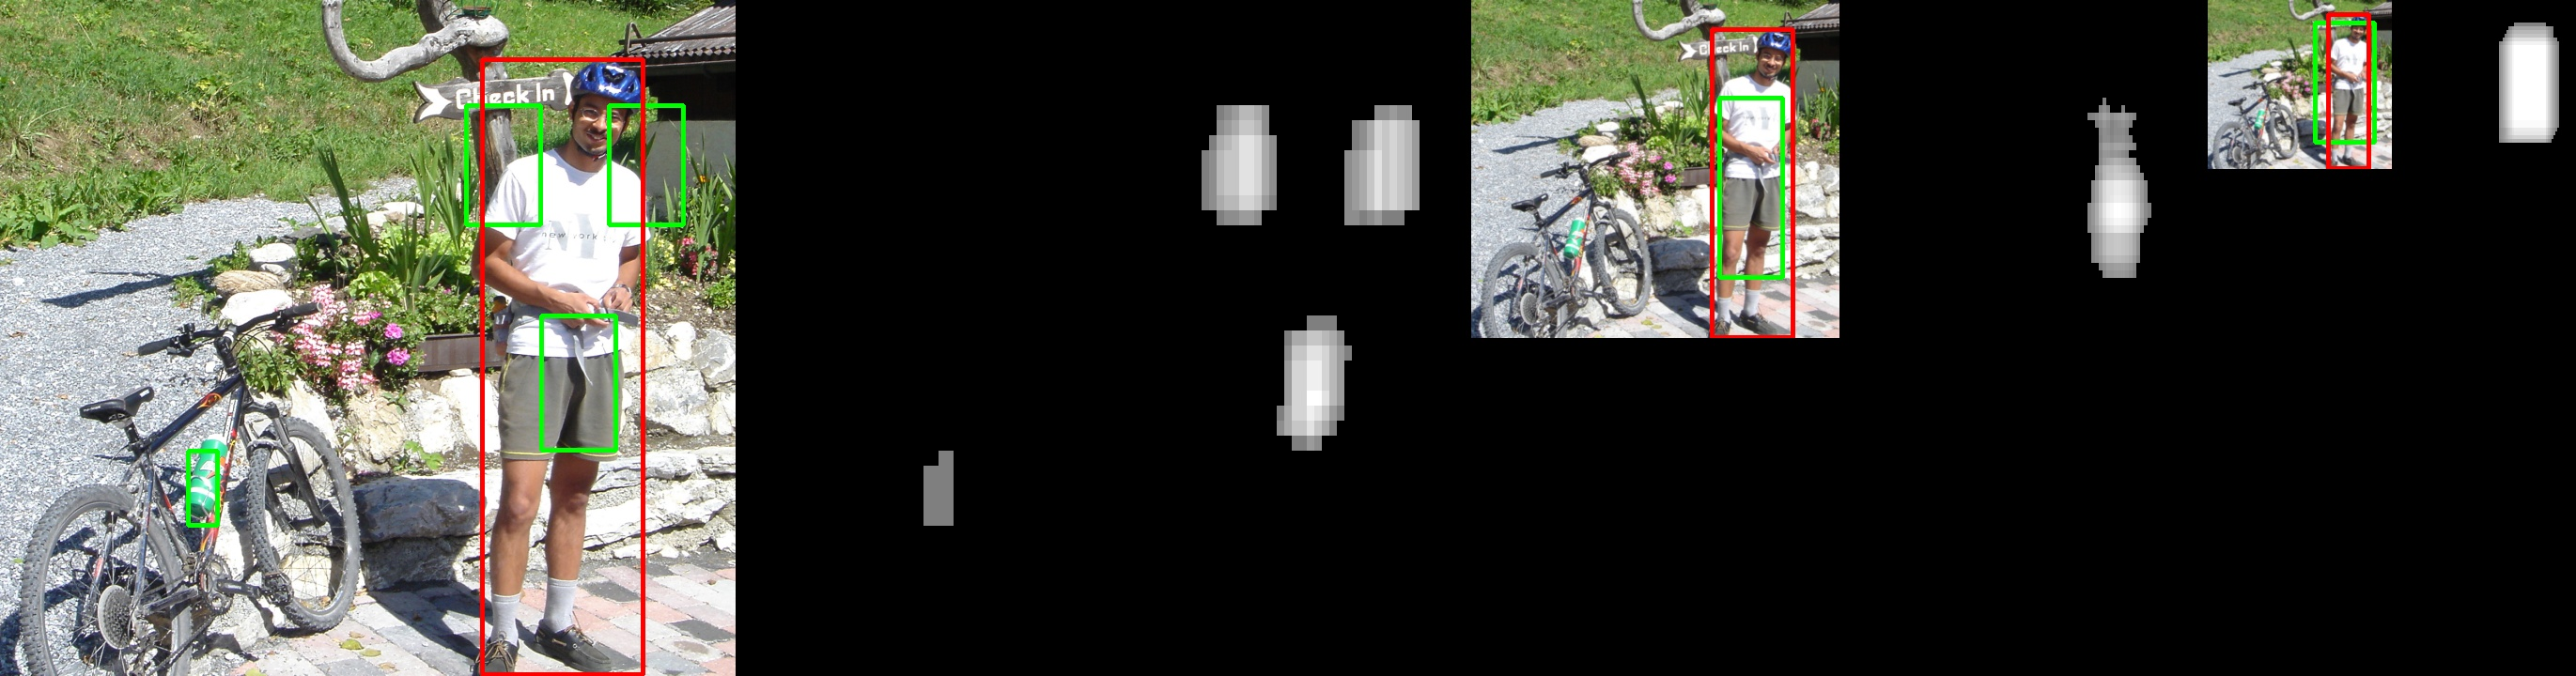
\includegraphics[scale=0.16]{./Imagenes/test01.jpg}
	\caption{Ejemplo de una persona junto a una bicicleta}
\end{figure}

En este ejemplo podemos ver cada uno de los tres niveles de la pirámide Gaussiana en los que tenemos marcadas cajas de color rojo y verde. Las cajas de color rojo son las provistas por el fichero de anotaciones de dicha imagen y las cajas verdes se corresponden con las halladas mediante el mapa de calor correspondiente. Además, se puede observar que el mapa de calor correspondiente a cada nivel se sitúa a la derecha de su imagen asociada.

Con esta información dada podemos observar en primer lugar las ventajas que vamos a obtener de usar el método de supresión de no máximos. Como podemos ver en el primer nivel de la pirámide Gaussiana hemos obtenido cuatro regiones en total y tres regiones muy próximas entre sí. Lo que hemos conseguido es que esas regiones se separen entre sí. Si no hubiéramos realizado la supresión tendríamos valores menores que el umbral rodeando dichas regiones, haciendo por tanto que el método obtuviera una única región. En este caso el hecho de obtener tres regiones no nos ha supuesto una ventaja, pero si pensamos en esta circunstancia cuando tengamos un grupo de peatones juntos podemos entender que gracias a esto es más fácil poder conseguir una caja para cada uno de ellos. 

Además aquí podemos ver también la potencia del uso de varios niveles de la pirámide Gaussiana. Al obtener una imagen de tamaño la mitad con respecto a la original tenemos que la ventana de $64\times 128$ que vamos pasando por la misma cubre una región mayor, con lo que es más propicia a que en niveles más bajos de la pirámide englobemos a peatones de tamaño grande en proporción a la imagen completa. Esto hace que el método que estamos empleando sea muy versátil, pues empleamos los niveles más altos de la pirámide para detectar peatones de pequeño tamaño por la misma y los niveles más bajos para los peatones de tamaño mayor.

Observemos el siguiente caso de estudio:

\begin{figure}[H]
	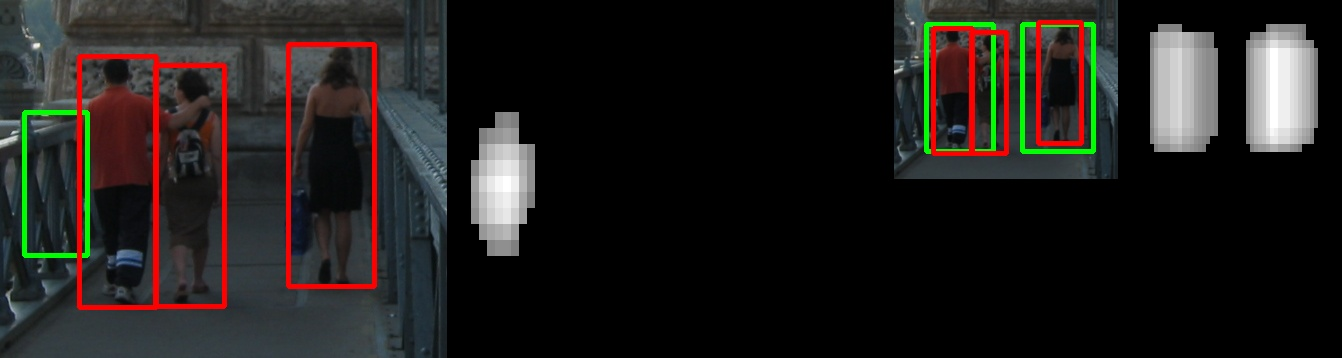
\includegraphics[scale=0.3]{./Imagenes/test02.jpg}
	\caption{Imagen de dos personas abrazadas y una andando al lado}
\end{figure}

En este caso podemos ver el ejemplo de tres peatones en un puente andando, estando dos de ellos muy pegados ya que van abrazados. Si analizamos el comportamiento nos damos cuenta de que los peatones en la imagen inicial ocupan un espacio muy significativo de la misma, por lo que el en primer nivel de la pirámide Gaussiana no hemos podido obtener unas cajas relevantes usando nuestra ventana. Este hecho no es así cuando pasamos al siguiente nivel, donde ya obtenemos dos cajas perfectamente delimitadas incluyendo a los peatones. 

Este hecho es importante puesto que en el ejemplo hemos podido separar dos regiones, la que contiene a los peatones abrazados y la que contiene al peatón que anda al lado. Esto es completamente razonable, ya que los peatones abrazados están tan juntos que nuestro umbral de supresión de no máximos no es capaz de discernir la división entre las regiones. Además no querríamos tener que aumentar tanto el nivel del umbral para conseguir la diferenciación, puesto que si lo hiciéramos nos quedaríamos con demasiados pocos valores en las regiones del mapa de calor, con lo que las ventanas obtenidas serían de un tamaño menor y por tanto no conseguiríamos el solapamiento del 50\% que vamos buscando. 

Veamos un ejemplo de dos personas con un espacio considerable entre sí para analizar una casuística favorable:

\begin{figure}[H]
	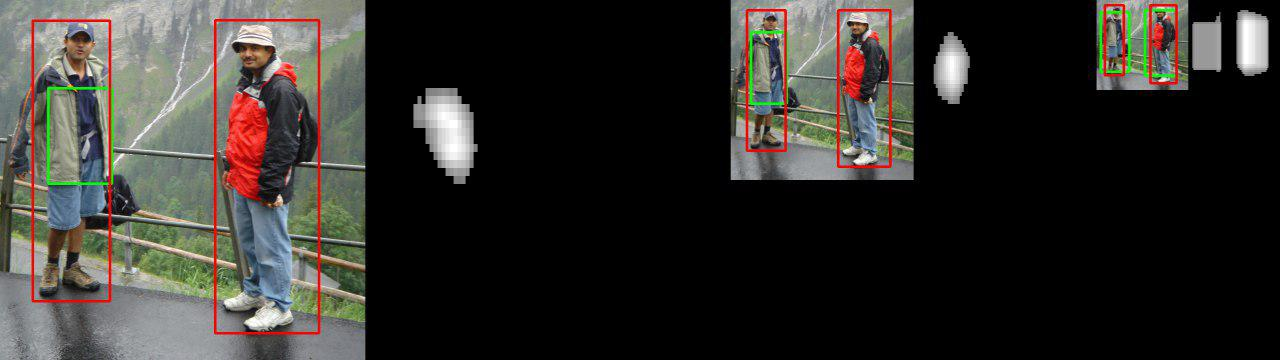
\includegraphics[scale=0.43]{./Imagenes/test03.jpg}
	\caption{Imagen de dos personas con una separación notable entre ellos}
\end{figure}

Como podemos observar esta casuística nos deja un espacio entre peatones que posibilita una distinción de las regiones muy evidente.

Veamos ahora un ejemplo aún más difícil con una alta concentración de personas:

\begin{figure}[H]
	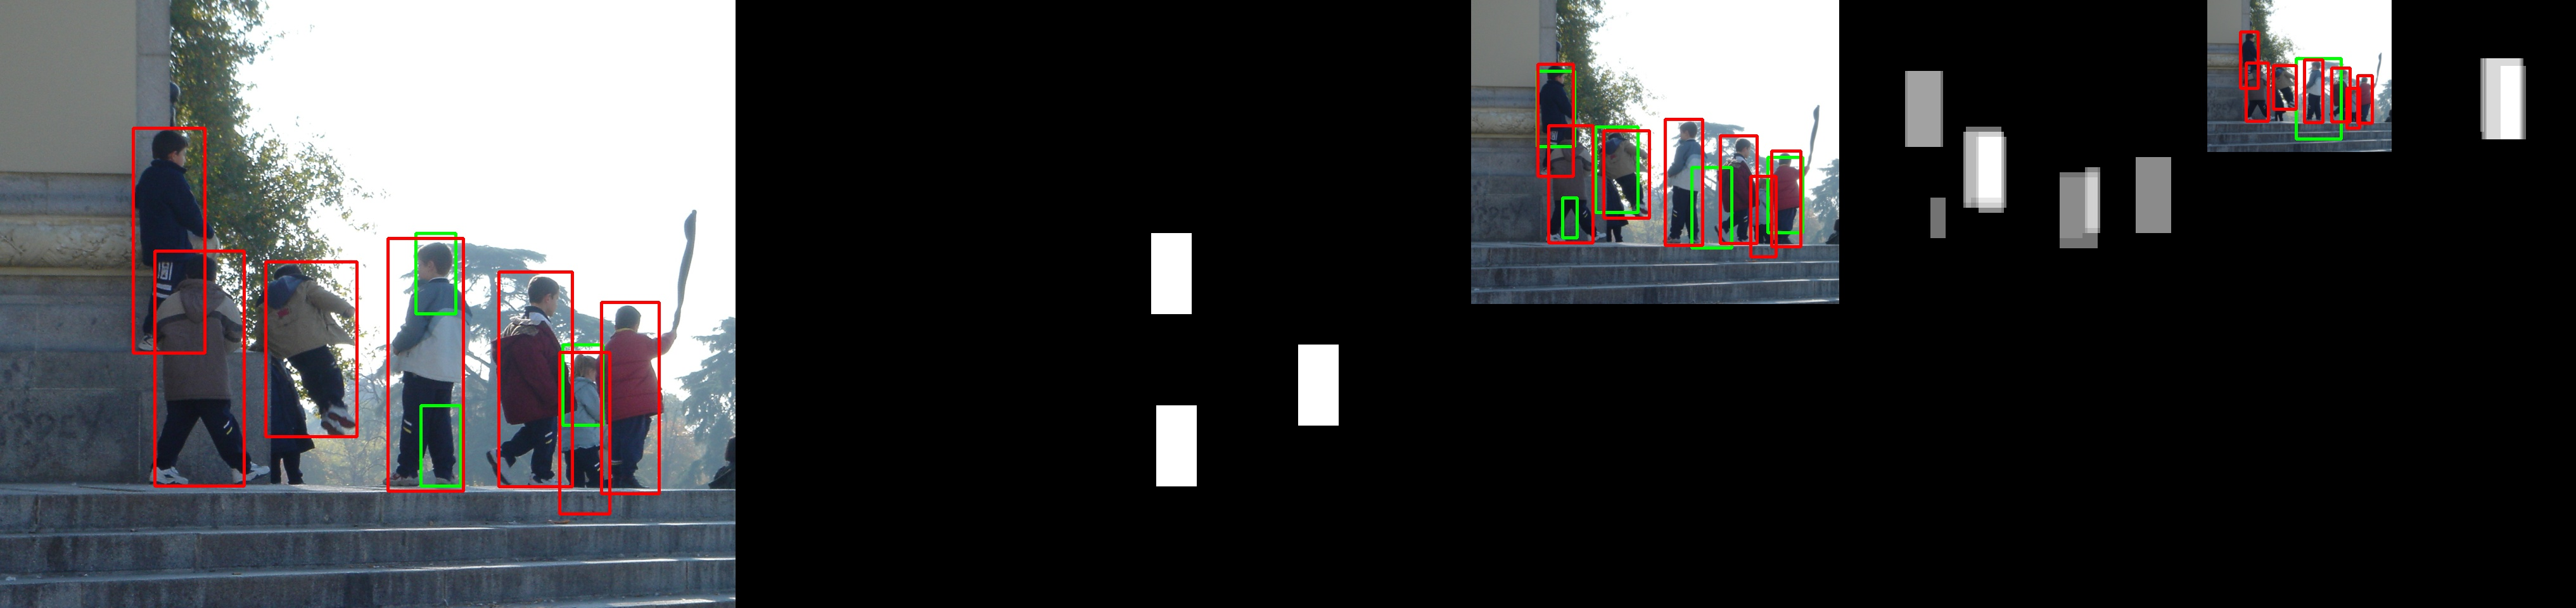
\includegraphics[scale=0.11]{./Imagenes/test04.jpg}
	\caption{Imagen de unos niños y personas andando}
\end{figure}

Esta imagen representa un salto en dificultad debido a la concentración de personas en la misma, en concreto tenemos 7 personas incluyendo a niños y personas de fondo. Como podemos observar el primer nivel de la pirámide no es útil debido al tamaño de las personas de la foto, por contra en el segundo nivel obtenemos unas ventanas muy favorables y si contamos las del segundo nivel y las del tercero entonces podemos comprobar que cubrimos casi todos los peatones de la imagen. Cabe destacar que no es simple la detección de todas estas personas. Representa un problema no sólo para el método si no también para los descriptores y la SVM puesto que los gradientes pueden variar enormemente si tenemos personas superpuestas entre sí.

\subsection{Métricas y resultados}

Para estudiar el funcionamiento del método de test hemos tomado varias métricas. Para las imágenes positivas hemos realizado en primer lugar una medición del acierto de peatones por imagen, de forma que obtenemos un número entre 0 y 1 que es $\frac{aciertos}{numero \ total \ de \ peatones}$ de forma que obtenemos un vector en el que en cada posición tenemos un número entre 0 y 1 con el acierto de peatones por imagen. De esta forma cuando obtenemos todos los resultados podemos sumarlos. La máxima puntuación que podríamos obtener en esta métrica es el número de imágenes. Esto nos deja la posibilidad de obtener un porcentaje de acierto medio por imagen. 

Además de esta métrica hemos incorporado otra que contabiliza, de forma global, cuántos peatones hemos acertado respecto a cuántos hay en total. De esta forma obtenemos $\frac{peatones \ acertados}{numero \ total \ de \ peatones}$. De igual forma podemos obtener un porcentaje con esta medida.

Para las imágenes negativas obtenemos una medida similar a la primera obtenida con las imágenes positivas. Esto es el número de ventanas acertadas por imagen partido por el número de ventanas por imagen. De esta forma obtenemos igualmente un valor entre 0 y 1 con lo que podemos hacer igual que con las imágenes positivas y obtener un porcentaje. 

Con esto los resultados que hemos obtenido son:

%%%%%%%%%%%%%%%%%%%%%%%%%%%%%%%%%%%%%%%%%%%%%%%%%%%%%%%%%%%%%%%%%%%%%%%%%%%%%%%%%%%%%%
%%                               Propuestas de mejora                               %%
%%%%%%%%%%%%%%%%%%%%%%%%%%%%%%%%%%%%%%%%%%%%%%%%%%%%%%%%%%%%%%%%%%%%%%%%%%%%%%%%%%%%%%



\subsection{Trabajo futuro: propuestas de mejora}

A pesar de que estamos contentos con el resultado obtenido. Despues del trabajo realizado podemos afirmar que nuestra implementacion tiene espacio para la mejora.

En primer lugar pensamos que el tiempo en el que se calculan los descriptores deberia ser mas razonable. Esto lo pensamos porque la aplicacion inmediata de una solucion como esta puede ser la identificacion de peatones desde un coche en conduccion. Teniendo en cuenta el tiempo que se tarda en identificar un peaton en una imagen (hay que recorrer los tres piramides de la piramide Gaussiana) no parece una opcion viable para la identificacion a tiempo real.

Otro hecho que identificamos como un problema es que este metodo es sensible al tamano de los peatones de la imagen. La forma que hemos tenido de paliar este hecho ha sido recorrer varios niveles de la piramide Gaussiana, a pesar de todo no esta asegurado que la ventana se adapte al tamano del peaton.

En ultimo lugar pensamos que el metodo de busqueda que utilizamos plantea una desventaja clara. Al acumular votos sobre un mapa de calor de una imagen ocurre que cuando los peatones se encuentran en puntos muy cercanos de la imagen las regiones que aparecen en el mapa de calor se solapan. Esto dificulta nuestra capacidad de
distinguir cada peaton como una entidad diferenciada.

\normalsize


% Bibliografía.
%-----------------------------------------------------------------
%\onecolumn
%\bibliography{referencias}
%\bibliographystyle{plain}
%\nocite{*}

\end{document}
